\documentclass{whiteboard}
\begin{document}
\begin{frame}[plain,t]
\bbcover{OBI 2008 - Nível 2: Fase 1}{Telefone}{Prof. Edson Alves}{Faculdade UnB Gama}

\end{frame}
\begin{frame}[plain,t]
\vspace*{\fill}

\bbtext{As primeiras redes públicas de telefonia foram construídas pela AT\&T; no começo do século XX. Elas permitiam que seus assinantes conversassem com a ajuda de uma telefonista, que conectava as linhas dos assinantes com um cabo especial.}

\vspace{0.1in}

\bbtext{Essas redes evoluíram muito desde então, com a ajuda de vários avanços tecnológicos. Hoje em dia, essas redes atendem centenas de milhões de assinantes; ao invés de falar diretamente com uma telefonista, você pode simplesmente discar o número da pessoa desejada no telefone.}

\vspace{0.1in}

\bbtext{Cada assinante recebe um número de telefone -- por exemplo, 55-98-234-5678. Qualquer pessoa que discar esse número consegue então falar com a pessoa do outro lado da linha. Os hifens no número de telefone são só para facilitar a leitura, e não são discados no telefone.}

\vspace{0.1in}

\bbtext{Para que fique mais fácil de se lembrar de um número de telefone, muitas companhias divulgam números que contém letras no lugar de dígitos. Para convertê-los de volta para dígitos, a maioria dos telefones tem letras nas suas teclas:}

\vspace*{\fill}
\end{frame}
\begin{frame}[plain,t]
\vspace*{\fill}

\begin{center}
\includegraphics[scale=0.8]{telefone.png}
\end{center}

\bbtext{Ao invés de discar uma letra, disca-se a tecla que contém aquela letra. Por exemplo, se você quiser discar o número 0800-FALE-SBC, você na realidade discaria 0800-3253-722.}

\vspace{0.1in}

\bbtext{A sua avó tem reclamado de problemas de vista -- em particular, ela não consegue mais enxergar as letrinhas nas teclas do telefone, e por isso queria que você fizesse um programa que convertesse as letras em um número de telefone para dígitos.}

\vspace*{\fill}
\end{frame}
\begin{frame}[plain,t]
\vspace*{\fill}

\bbbold{Entrada}

\vspace{0.2in}

\bbtext{A primeira linha da entrada contém um inteiro $N$, o número de valores sorteados. A segunda linha contém $N$
valores, $V_1, V_2, \ldots, V_N$, na ordem de sorteio, separados por um espaço em branco.}

\vspace{0.2in}

\bbbold{Saída}

\vspace{0.2in}

\bbtext{Seu programa deve imprimir apenas uma linha, contendo apenas um inteiro, indicando o número de pontos do
participante.}

\vspace{0.2in}

\bbbold{Restrições}
\vspace{-0.1in}

\bbtext{
\begin{itemize}
\item $1\leq N\leq 10^4$
\item $-2^{31}\leq V_i\leq 2^{31} - 1$\bbtext{, para} $i = 1, 2, \ldots, N$
\end{itemize}
}
\vspace*{\fill}
\end{frame}
\begin{frame}[plain,t]
\begin{tikzpicture}
\node[draw,opacity=0] at (0, 0) {x};
\node[draw,opacity=0] at (14, 8) {x};

	\node[anchor=west] (header) at (0, 7.0) { \bbbold{Exemplo de entrada e saída} };

\end{tikzpicture}
\end{frame}
\begin{frame}[plain,t]
\begin{tikzpicture}
\node[draw,opacity=0] at (0, 0) {x};
\node[draw,opacity=0] at (14, 8) {x};

	\node[anchor=west] (header) at (0, 7.0) { \bbbold{Exemplo de entrada e saída} };


	\node[anchor=west] (line1) at (1.0, 6.0) { \bbtext{\texttt{11} } };

\end{tikzpicture}
\end{frame}
\begin{frame}[plain,t]
\begin{tikzpicture}
\node[draw,opacity=0] at (0, 0) {x};
\node[draw,opacity=0] at (14, 8) {x};

	\node[anchor=west] (header) at (0, 7.0) { \bbbold{Exemplo de entrada e saída} };


	\node[anchor=west] (line1) at (1.0, 6.0) { \bbtext{\texttt{11} } };


	\draw[->,color=BBViolet] (1.35, 5.0) to  (1.35, 5.75);

	\node[anchor=west] (r) at (0.5, 4.75) { \footnotesize \bbcomment{\# de valores sorteados} };

\end{tikzpicture}
\end{frame}
\begin{frame}[plain,t]
\begin{tikzpicture}
\node[draw,opacity=0] at (0, 0) {x};
\node[draw,opacity=0] at (14, 8) {x};

	\node[anchor=west] (header) at (0, 7.0) { \bbbold{Exemplo de entrada e saída} };


	\node[anchor=west] (line1) at (1.0, 6.0) { \bbtext{\texttt{11} } };





	\node[anchor=west] (line2) at (1.0, 5.5) { \bbtext{\texttt{30 30 30 30 40 40 40 40 40 30 30}} };

\end{tikzpicture}
\end{frame}
\begin{frame}[plain,t]
\begin{tikzpicture}
\node[draw,opacity=0] at (0, 0) {x};
\node[draw,opacity=0] at (14, 8) {x};

	\node[anchor=west] (header) at (0, 7.0) { \bbbold{Exemplo de entrada e saída} };


	\node[anchor=west] (line1) at (1.0, 6.0) { \bbtext{\texttt{11} } };


	\draw[->,color=BBViolet] (4.35, 5.0) to  (4.35, 3.75);

	\node[anchor=west] (r) at (3.25, 3.25) { \footnotesize \bbcomment{Números sorteados} };


	\node[anchor=west] (line2) at (1.0, 5.5) { \bbtext{\texttt{30 30 30 30 40 40 40 40 40 30 30}} };





\end{tikzpicture}
\end{frame}
\begin{frame}[plain,t]
\begin{tikzpicture}
\node[draw,opacity=0] at (0, 0) {x};
\node[draw,opacity=0] at (14, 8) {x};

	\node[anchor=west] (header) at (0, 7.0) { \bbbold{Exemplo de entrada e saída} };


	\node[anchor=west] (line1) at (1.0, 6.0) { \bbtext{\texttt{11} } };





	\node[anchor=west] (line2) at (1.0, 5.5) { \bbtext{\texttt{30 30 30 30 40 40 40 40 40 30 30}} };







	\node[draw,very thick,circle] (node1) at (2.0, 3.0) { \bbtext{\texttt{30}} };

	\node[draw,very thick,circle] (node2) at (3.0, 3.0) { \bbtext{\texttt{30}} };

	\node[draw,very thick,circle] (node3) at (4.0, 3.0) { \bbtext{\texttt{30}} };

	\node[draw,very thick,circle] (node4) at (5.0, 3.0) { \bbtext{\texttt{30}} };

	\node[draw,very thick,circle] (node5) at (6.0, 3.0) { \bbtext{\texttt{40}} };

	\node[draw,very thick,circle] (node6) at (7.0, 3.0) { \bbtext{\texttt{40}} };

	\node[draw,very thick,circle] (node7) at (8.0, 3.0) { \bbtext{\texttt{40}} };

	\node[draw,very thick,circle] (node8) at (9.0, 3.0) { \bbtext{\texttt{40}} };

	\node[draw,very thick,circle] (node9) at (10.0, 3.0) { \bbtext{\texttt{40}} };

	\node[draw,very thick,circle] (node10) at (11.0, 3.0) { \bbtext{\texttt{30}} };

	\node[draw,very thick,circle] (node11) at (12.0, 3.0) { \bbtext{\texttt{30}} };

\end{tikzpicture}
\end{frame}
\begin{frame}[plain,t]
\begin{tikzpicture}
\node[draw,opacity=0] at (0, 0) {x};
\node[draw,opacity=0] at (14, 8) {x};

	\node[anchor=west] (header) at (0, 7.0) { \bbbold{Exemplo de entrada e saída} };


	\node[anchor=west] (line1) at (1.0, 6.0) { \bbtext{\texttt{11} } };





	\node[anchor=west] (line2) at (1.0, 5.5) { \bbtext{\texttt{30 30 30 30 40 40 40 40 40 30 30}} };







	\node[draw,very thick,circle,fill=BBGreen] (node1) at (2.0, 3.0) { \bbtext{\texttt{30}} };

	\node[draw,very thick,circle,fill=BBGreen] (node2) at (3.0, 3.0) { \bbtext{\texttt{30}} };

	\node[draw,very thick,circle,fill=BBGreen] (node3) at (4.0, 3.0) { \bbtext{\texttt{30}} };

	\node[draw,very thick,circle,fill=BBGreen] (node4) at (5.0, 3.0) { \bbtext{\texttt{30}} };

	\node[draw,very thick,circle] (node5) at (6.0, 3.0) { \bbtext{\texttt{40}} };

	\node[draw,very thick,circle] (node6) at (7.0, 3.0) { \bbtext{\texttt{40}} };

	\node[draw,very thick,circle] (node7) at (8.0, 3.0) { \bbtext{\texttt{40}} };

	\node[draw,very thick,circle] (node8) at (9.0, 3.0) { \bbtext{\texttt{40}} };

	\node[draw,very thick,circle] (node9) at (10.0, 3.0) { \bbtext{\texttt{40}} };

	\node[draw,very thick,circle] (node10) at (11.0, 3.0) { \bbtext{\texttt{30}} };

	\node[draw,very thick,circle] (node11) at (12.0, 3.0) { \bbtext{\texttt{30}} };



\end{tikzpicture}
\end{frame}
\begin{frame}[plain,t]
\begin{tikzpicture}
\node[draw,opacity=0] at (0, 0) {x};
\node[draw,opacity=0] at (14, 8) {x};

	\node[anchor=west] (header) at (0, 7.0) { \bbbold{Exemplo de entrada e saída} };


	\node[anchor=west] (line1) at (1.0, 6.0) { \bbtext{\texttt{11} } };





	\node[anchor=west] (line2) at (1.0, 5.5) { \bbtext{\texttt{30 30 30 30 40 40 40 40 40 30 30}} };







	\node[draw,very thick,circle,fill=BBWhite] (node1) at (2.0, 3.0) { \bbtext{\texttt{30}} };

	\node[draw,very thick,circle,fill=BBWhite] (node2) at (3.0, 3.0) { \bbtext{\texttt{30}} };

	\node[draw,very thick,circle,fill=BBWhite] (node3) at (4.0, 3.0) { \bbtext{\texttt{30}} };

	\node[draw,very thick,circle,fill=BBWhite] (node4) at (5.0, 3.0) { \bbtext{\texttt{30}} };

	\node[draw,very thick,circle,fill=BBCyan] (node5) at (6.0, 3.0) { \bbtext{\texttt{40}} };

	\node[draw,very thick,circle,fill=BBCyan] (node6) at (7.0, 3.0) { \bbtext{\texttt{40}} };

	\node[draw,very thick,circle,fill=BBCyan] (node7) at (8.0, 3.0) { \bbtext{\texttt{40}} };

	\node[draw,very thick,circle,fill=BBCyan] (node8) at (9.0, 3.0) { \bbtext{\texttt{40}} };

	\node[draw,very thick,circle,fill=BBCyan] (node9) at (10.0, 3.0) { \bbtext{\texttt{40}} };

	\node[draw,very thick,circle] (node10) at (11.0, 3.0) { \bbtext{\texttt{30}} };

	\node[draw,very thick,circle] (node11) at (12.0, 3.0) { \bbtext{\texttt{30}} };






\end{tikzpicture}
\end{frame}
\begin{frame}[plain,t]
\begin{tikzpicture}
\node[draw,opacity=0] at (0, 0) {x};
\node[draw,opacity=0] at (14, 8) {x};

	\node[anchor=west] (header) at (0, 7.0) { \bbbold{Exemplo de entrada e saída} };


	\node[anchor=west] (line1) at (1.0, 6.0) { \bbtext{\texttt{11} } };





	\node[anchor=west] (line2) at (1.0, 5.5) { \bbtext{\texttt{30 30 30 30 40 40 40 40 40 30 30}} };







	\node[draw,very thick,circle,fill=BBWhite] (node1) at (2.0, 3.0) { \bbtext{\texttt{30}} };

	\node[draw,very thick,circle,fill=BBWhite] (node2) at (3.0, 3.0) { \bbtext{\texttt{30}} };

	\node[draw,very thick,circle,fill=BBWhite] (node3) at (4.0, 3.0) { \bbtext{\texttt{30}} };

	\node[draw,very thick,circle,fill=BBWhite] (node4) at (5.0, 3.0) { \bbtext{\texttt{30}} };

	\node[draw,very thick,circle,fill=BBWhite] (node5) at (6.0, 3.0) { \bbtext{\texttt{40}} };

	\node[draw,very thick,circle,fill=BBWhite] (node6) at (7.0, 3.0) { \bbtext{\texttt{40}} };

	\node[draw,very thick,circle,fill=BBWhite] (node7) at (8.0, 3.0) { \bbtext{\texttt{40}} };

	\node[draw,very thick,circle,fill=BBWhite] (node8) at (9.0, 3.0) { \bbtext{\texttt{40}} };

	\node[draw,very thick,circle,fill=BBWhite] (node9) at (10.0, 3.0) { \bbtext{\texttt{40}} };

	\node[draw,very thick,circle,fill=BBOrange] (node10) at (11.0, 3.0) { \bbtext{\texttt{30}} };

	\node[draw,very thick,circle,fill=BBOrange] (node11) at (12.0, 3.0) { \bbtext{\texttt{30}} };









\end{tikzpicture}
\end{frame}
\begin{frame}[plain,t]
\begin{tikzpicture}
\node[draw,opacity=0] at (0, 0) {x};
\node[draw,opacity=0] at (14, 8) {x};

	\node[anchor=west] (header) at (0, 7.0) { \bbbold{Exemplo de entrada e saída} };


	\node[anchor=west] (line1) at (1.0, 6.0) { \bbtext{\texttt{11} } };


	\draw[->,color=BBBlack,-latex,thick] (8.0, 5.5) to  (10.0, 5.5);

	\node[anchor=west] (r) at (10.25, 5.5) { \footnotesize \bboutput{5} };


	\node[anchor=west] (line2) at (1.0, 5.5) { \bbtext{\texttt{30 30 30 30 40 40 40 40 40 30 30}} };







	\node[draw,very thick,circle,fill=BBWhite] (node1) at (2.0, 3.0) { \bbtext{\texttt{30}} };

	\node[draw,very thick,circle,fill=BBWhite] (node2) at (3.0, 3.0) { \bbtext{\texttt{30}} };

	\node[draw,very thick,circle,fill=BBWhite] (node3) at (4.0, 3.0) { \bbtext{\texttt{30}} };

	\node[draw,very thick,circle,fill=BBWhite] (node4) at (5.0, 3.0) { \bbtext{\texttt{30}} };

	\node[draw,very thick,circle,fill=BBWhite] (node5) at (6.0, 3.0) { \bbtext{\texttt{40}} };

	\node[draw,very thick,circle,fill=BBWhite] (node6) at (7.0, 3.0) { \bbtext{\texttt{40}} };

	\node[draw,very thick,circle,fill=BBWhite] (node7) at (8.0, 3.0) { \bbtext{\texttt{40}} };

	\node[draw,very thick,circle,fill=BBWhite] (node8) at (9.0, 3.0) { \bbtext{\texttt{40}} };

	\node[draw,very thick,circle,fill=BBWhite] (node9) at (10.0, 3.0) { \bbtext{\texttt{40}} };

	\node[draw,very thick,circle,fill=BBOrange] (node10) at (11.0, 3.0) { \bbtext{\texttt{30}} };

	\node[draw,very thick,circle,fill=BBOrange] (node11) at (12.0, 3.0) { \bbtext{\texttt{30}} };














\end{tikzpicture}
\end{frame}
\begin{frame}[plain,t]
\begin{tikzpicture}
\node[draw,opacity=0] at (0, 0) {x};
\node[draw,opacity=0] at (14, 8) {x};

	\node[anchor=west] (title) at (0.0, 7.0) { \Large \bbbold{Solução} };

\end{tikzpicture}
\end{frame}
\begin{frame}[plain,t]
\begin{tikzpicture}
\node[draw,opacity=0] at (0, 0) {x};
\node[draw,opacity=0] at (14, 8) {x};

	\node[anchor=west] (title) at (0.0, 7.0) { \Large \bbbold{Solução} };


	\node[anchor=west] (a) at (1.0, 6.0) { $\star$ \bbtext{O problema consiste em identificar as sequências de números consecutivos} };

\end{tikzpicture}
\end{frame}
\begin{frame}[plain,t]
\begin{tikzpicture}
\node[draw,opacity=0] at (0, 0) {x};
\node[draw,opacity=0] at (14, 8) {x};

	\node[anchor=west] (title) at (0.0, 7.0) { \Large \bbbold{Solução} };


	\node[anchor=west] (a) at (1.0, 6.0) { $\star$ \bbtext{O problema consiste em identificar as sequências de números consecutivos} };


	\node[anchor=west] (b) at (1.0, 5.0) { $\star$ \bbtext{Uma vez identificadas, a resposta será o tamanho da maior delas} };

\end{tikzpicture}
\end{frame}
\begin{frame}[plain,t]
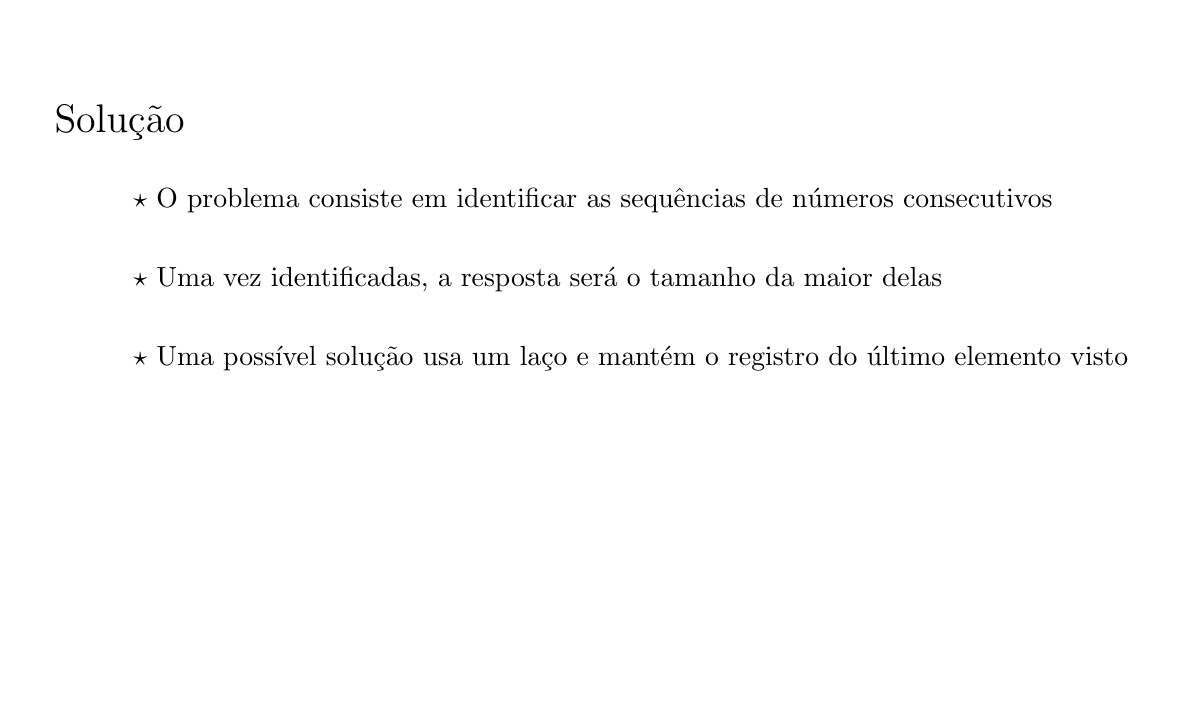
\begin{tikzpicture}
\node[draw,opacity=0] at (0, 0) {x};
\node[draw,opacity=0] at (14, 8) {x};

	\node[anchor=west] (title) at (0.0, 7.0) { \Large \bbbold{Solução} };


	\node[anchor=west] (a) at (1.0, 6.0) { $\star$ \bbtext{O problema consiste em identificar as sequências de números consecutivos} };


	\node[anchor=west] (b) at (1.0, 5.0) { $\star$ \bbtext{Uma vez identificadas, a resposta será o tamanho da maior delas} };


	\node[anchor=west] (c) at (1.0, 4.0) { $\star$ \bbtext{Uma possível solução usa um laço e mantém o registro do último elemento visto} };

\end{tikzpicture}
\end{frame}
\begin{frame}[plain,t]
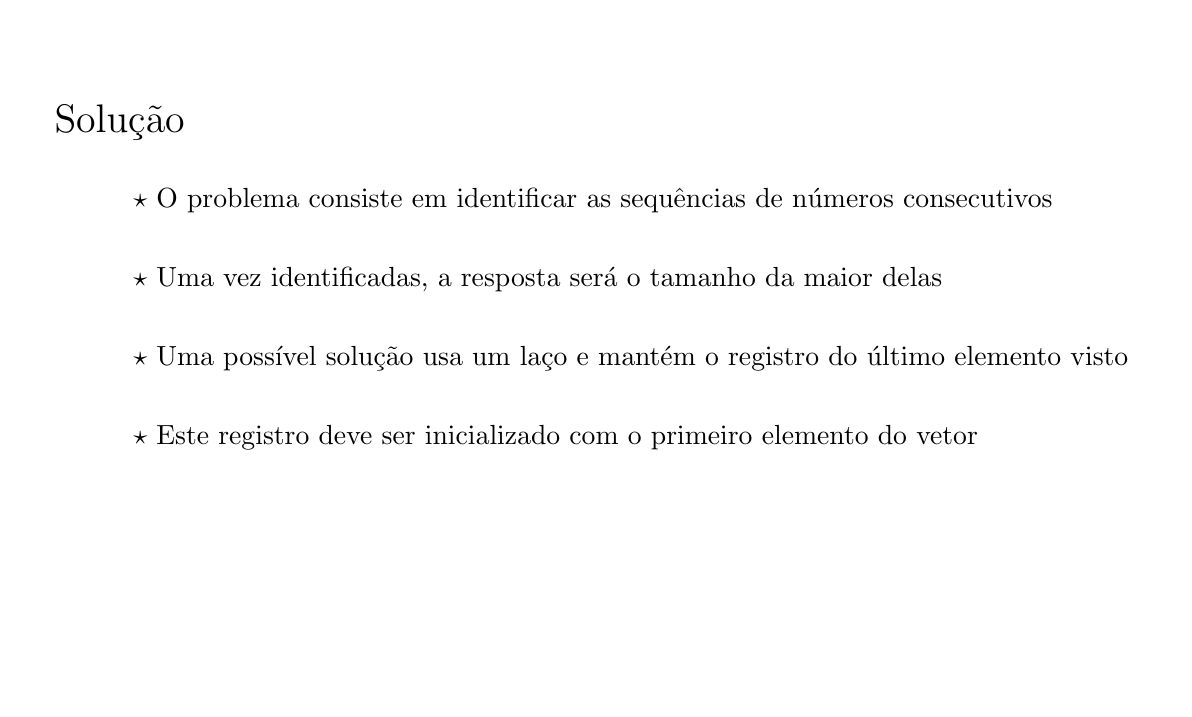
\begin{tikzpicture}
\node[draw,opacity=0] at (0, 0) {x};
\node[draw,opacity=0] at (14, 8) {x};

	\node[anchor=west] (title) at (0.0, 7.0) { \Large \bbbold{Solução} };


	\node[anchor=west] (a) at (1.0, 6.0) { $\star$ \bbtext{O problema consiste em identificar as sequências de números consecutivos} };


	\node[anchor=west] (b) at (1.0, 5.0) { $\star$ \bbtext{Uma vez identificadas, a resposta será o tamanho da maior delas} };


	\node[anchor=west] (c) at (1.0, 4.0) { $\star$ \bbtext{Uma possível solução usa um laço e mantém o registro do último elemento visto} };


	\node[anchor=west] (d) at (1.0, 3.0) { $\star$ \bbtext{Este registro deve ser inicializado com o primeiro elemento do vetor} };

\end{tikzpicture}
\end{frame}
\begin{frame}[plain,t]
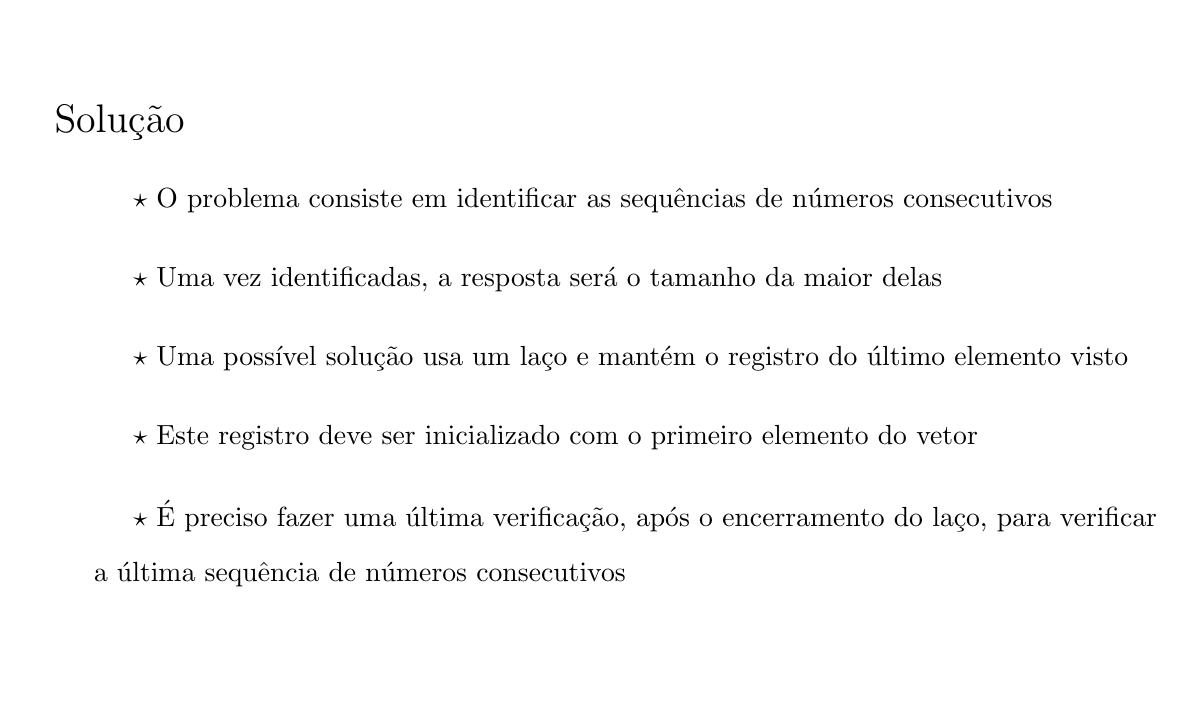
\begin{tikzpicture}
\node[draw,opacity=0] at (0, 0) {x};
\node[draw,opacity=0] at (14, 8) {x};

	\node[anchor=west] (title) at (0.0, 7.0) { \Large \bbbold{Solução} };


	\node[anchor=west] (a) at (1.0, 6.0) { $\star$ \bbtext{O problema consiste em identificar as sequências de números consecutivos} };


	\node[anchor=west] (b) at (1.0, 5.0) { $\star$ \bbtext{Uma vez identificadas, a resposta será o tamanho da maior delas} };


	\node[anchor=west] (c) at (1.0, 4.0) { $\star$ \bbtext{Uma possível solução usa um laço e mantém o registro do último elemento visto} };


	\node[anchor=west] (d) at (1.0, 3.0) { $\star$ \bbtext{Este registro deve ser inicializado com o primeiro elemento do vetor} };


	\node[anchor=west] (e) at (1.0, 2.0) { $\star$ \bbtext{É preciso fazer uma última verificação, após o encerramento do laço, para verificar} };

	\node[anchor=west] (e1) at (0.5, 1.25) { \bbtext{a última sequência de números consecutivos} };

\end{tikzpicture}
\end{frame}
\begin{frame}[plain,t]
\begin{tikzpicture}
\node[draw,opacity=0] at (0, 0) {x};
\node[draw,opacity=0] at (14, 8) {x};

	\node[anchor=west] (title) at (0.0, 7.0) { \Large \bbbold{Bônus} };

\end{tikzpicture}
\end{frame}
\begin{frame}[plain,t]
\begin{tikzpicture}
\node[draw,opacity=0] at (0, 0) {x};
\node[draw,opacity=0] at (14, 8) {x};

	\node[anchor=west] (title) at (0.0, 7.0) { \Large \bbbold{Bônus} };


	\node[anchor=west] (a) at (1.0, 6.0) { $\star$ \bbtext{Há uma solução alternativa para este problema} };

\end{tikzpicture}
\end{frame}
\begin{frame}[plain,t]
\begin{tikzpicture}
\node[draw,opacity=0] at (0, 0) {x};
\node[draw,opacity=0] at (14, 8) {x};

	\node[anchor=west] (title) at (0.0, 7.0) { \Large \bbbold{Bônus} };


	\node[anchor=west] (a) at (1.0, 6.0) { $\star$ \bbtext{Há uma solução alternativa para este problema} };


	\node[anchor=west] (b) at (1.0, 5.0) { $\star$ \bbtext{Ela é baseada em uma técnica denominada \bbbold{dois ponteiros}} };

\end{tikzpicture}
\end{frame}
\begin{frame}[plain,t]
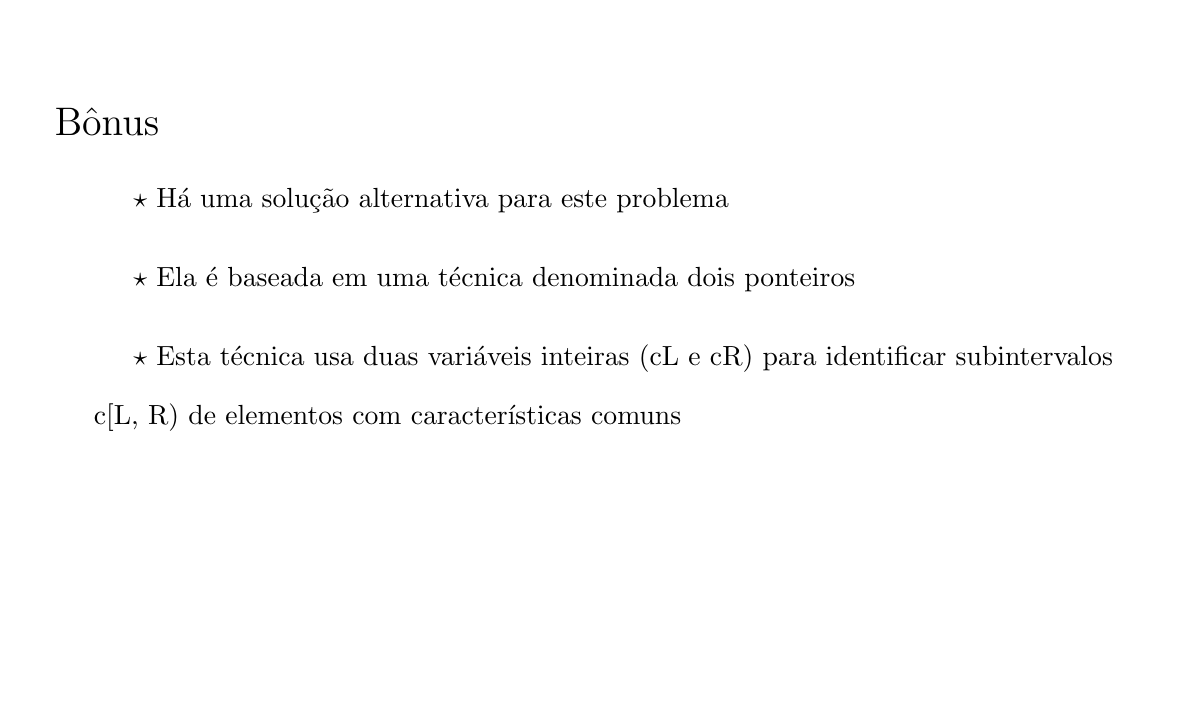
\begin{tikzpicture}
\node[draw,opacity=0] at (0, 0) {x};
\node[draw,opacity=0] at (14, 8) {x};

	\node[anchor=west] (title) at (0.0, 7.0) { \Large \bbbold{Bônus} };


	\node[anchor=west] (a) at (1.0, 6.0) { $\star$ \bbtext{Há uma solução alternativa para este problema} };


	\node[anchor=west] (b) at (1.0, 5.0) { $\star$ \bbtext{Ela é baseada em uma técnica denominada \bbbold{dois ponteiros}} };


	\node[anchor=west] (c) at (1.0, 4.0) { $\star$ \bbtext{Esta técnica usa duas variáveis inteiras (\code{c}{L} e \code{c}{R}) para identificar subintervalos} };

	\node[anchor=west] (c1) at (0.5, 3.25) { \bbtext{\code{c}{[L, R)} de elementos com características comuns} };

\end{tikzpicture}
\end{frame}
\begin{frame}[plain,t]
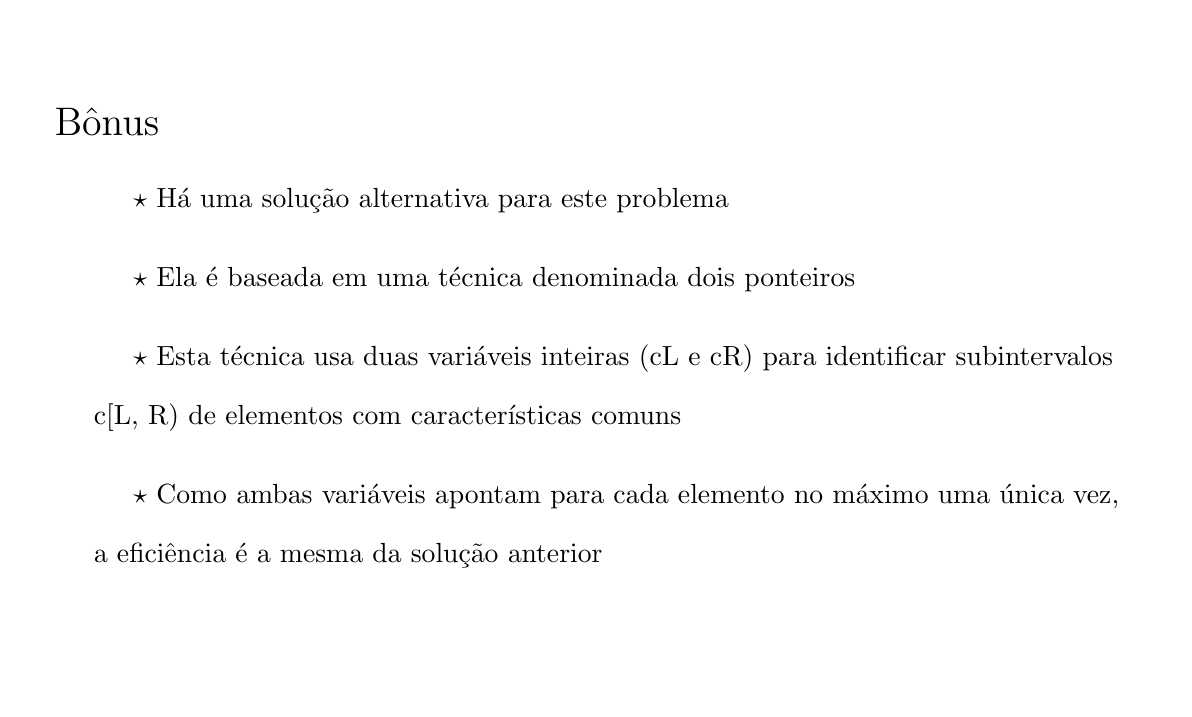
\begin{tikzpicture}
\node[draw,opacity=0] at (0, 0) {x};
\node[draw,opacity=0] at (14, 8) {x};

	\node[anchor=west] (title) at (0.0, 7.0) { \Large \bbbold{Bônus} };


	\node[anchor=west] (a) at (1.0, 6.0) { $\star$ \bbtext{Há uma solução alternativa para este problema} };


	\node[anchor=west] (b) at (1.0, 5.0) { $\star$ \bbtext{Ela é baseada em uma técnica denominada \bbbold{dois ponteiros}} };


	\node[anchor=west] (c) at (1.0, 4.0) { $\star$ \bbtext{Esta técnica usa duas variáveis inteiras (\code{c}{L} e \code{c}{R}) para identificar subintervalos} };

	\node[anchor=west] (c1) at (0.5, 3.25) { \bbtext{\code{c}{[L, R)} de elementos com características comuns} };


	\node[anchor=west] (d) at (1.0, 2.25) { $\star$ \bbtext{Como ambas variáveis apontam para cada elemento no máximo uma única vez, } };

	\node[anchor=west] (d1) at (0.5, 1.5) { \bbtext{a eficiência é a mesma da solução anterior} };

\end{tikzpicture}
\end{frame}
\begin{frame}[plain,t]
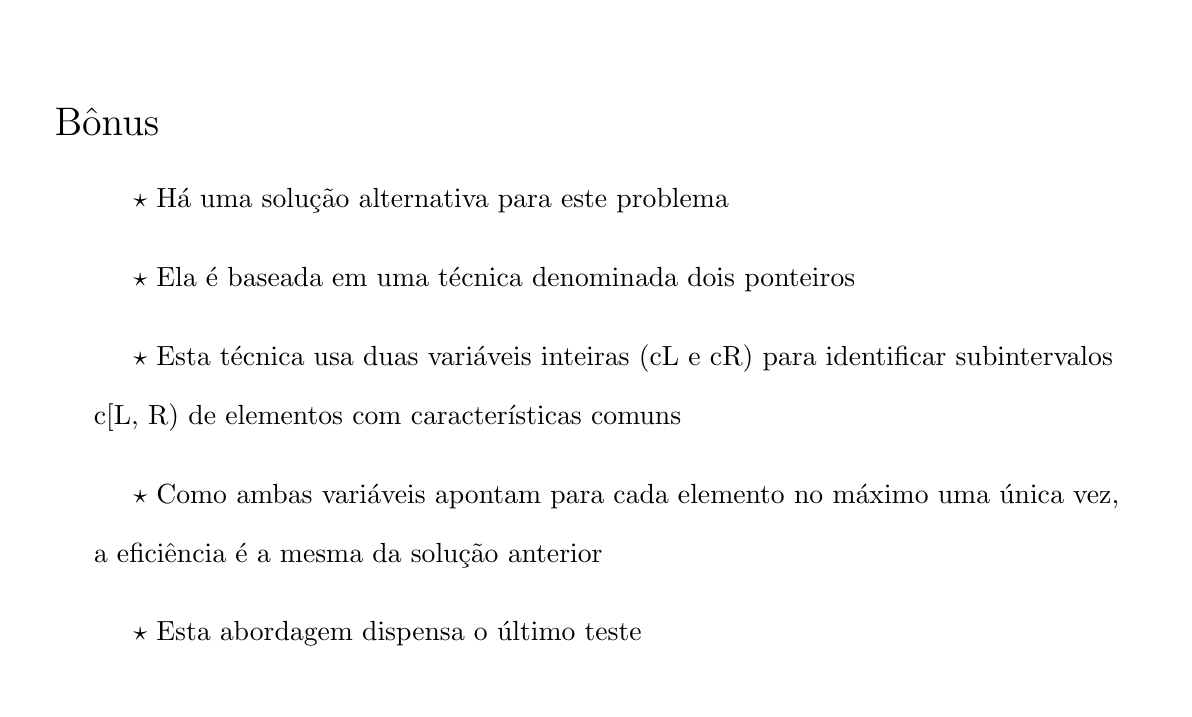
\begin{tikzpicture}
\node[draw,opacity=0] at (0, 0) {x};
\node[draw,opacity=0] at (14, 8) {x};

	\node[anchor=west] (title) at (0.0, 7.0) { \Large \bbbold{Bônus} };


	\node[anchor=west] (a) at (1.0, 6.0) { $\star$ \bbtext{Há uma solução alternativa para este problema} };


	\node[anchor=west] (b) at (1.0, 5.0) { $\star$ \bbtext{Ela é baseada em uma técnica denominada \bbbold{dois ponteiros}} };


	\node[anchor=west] (c) at (1.0, 4.0) { $\star$ \bbtext{Esta técnica usa duas variáveis inteiras (\code{c}{L} e \code{c}{R}) para identificar subintervalos} };

	\node[anchor=west] (c1) at (0.5, 3.25) { \bbtext{\code{c}{[L, R)} de elementos com características comuns} };


	\node[anchor=west] (d) at (1.0, 2.25) { $\star$ \bbtext{Como ambas variáveis apontam para cada elemento no máximo uma única vez, } };

	\node[anchor=west] (d1) at (0.5, 1.5) { \bbtext{a eficiência é a mesma da solução anterior} };


	\node[anchor=west] (e) at (1.0, 0.5) { $\star$ \bbtext{Esta abordagem dispensa o último teste} };

\end{tikzpicture}
\end{frame}
\end{document}
